\section{Learning Motion Primitive using Kinesthetic Demonstrations}
\label{sec:Learning motion primitive}
The main idea of the work is to infer the relevant set of features,
which describe the demonstrated motion primitive.
Based on the learnt relevant features, during the execution phase 
the robot tries to predict the goal of the motion primitive, starting 
from a new initial condition.

The demonstrations consist of recording two  states of the world
called as the start state and the end state.
So each demonstrations have 2 snapshots of the world in the initial state and the final state.
Based on these snapshots we try to infer the intent of the demonstrations. 

The motion primitive in our representation consist of pre-conditions and the post-conditions.
The execution of each motion primitive depends on the features used to explain it.
Each motion primitive is defined by a set of features which are a subset of the complete feature space, 
which are also relevant for the robot to execute the respective motion primitive.

\subsection{Features}
Features are the basic building block, which are used to describe a motion primitive.
A Feature $f$ can be defined as any quantitative parameter of the world $W$.
For example the pose of the robot, color of the box, distance between box and robot,
displacement of the tooltip in time.

Features are broadly classified into :
\begin{enumerate}
    \item features describing object properties $f(O)$
    \begin{enumerate}
        \item features describing robot properties $f(O_r)$ (eg : pose of the robot)
        \item features describing environment properties $f(O_e)$(eg: color of the box)
    \end{enumerate}
    \item features describing relation between object properties $g(O_1, O_2)$
    \begin{enumerate}
        \item relation between  different objects $g(O_1, O_2)$ (eg : distance between box and robot)
        \item relation between same object in time $g(O_{1i}, O_{1f}) $(eg : displacement of tooltip)
    \end{enumerate}
\end{enumerate}


Thus the collection of featues can be defined as 
\begin{equation}
    \begin{aligned}
    F &= f(O) + g(O_1 , O_2) \\
      &= (f(O_r) + f(O_e))  +  (g(O_1, O_2) + g(O_{1i}, O_{1f}))
    \end{aligned}
\end{equation}

As explained in section \ref{sec:Proposed motion primitive}
the proposed motion primitive is defined using pre and post conditions of the features.
\begin{equation}
    \begin{aligned}
    & \text{Motion primitive} := (f_s, f_e ) \\
    & where  \nonumber \\ 
    &    f_s = \text{features in start of demonstrations} \nonumber\\
    &    f_e = \text{features in end of demonstrations} \nonumber
    \end{aligned}
\end{equation}



\subsection{Modelling Motion Primitive}

The learning problem can be considered as a supervised learning problem, where 
the model has to learn from the set of demonstrations to predict the output
$f_e$ when a new input $f_s$ is provided as explained in figure \ref{model}.
\begin{figure}[htp]
\centering
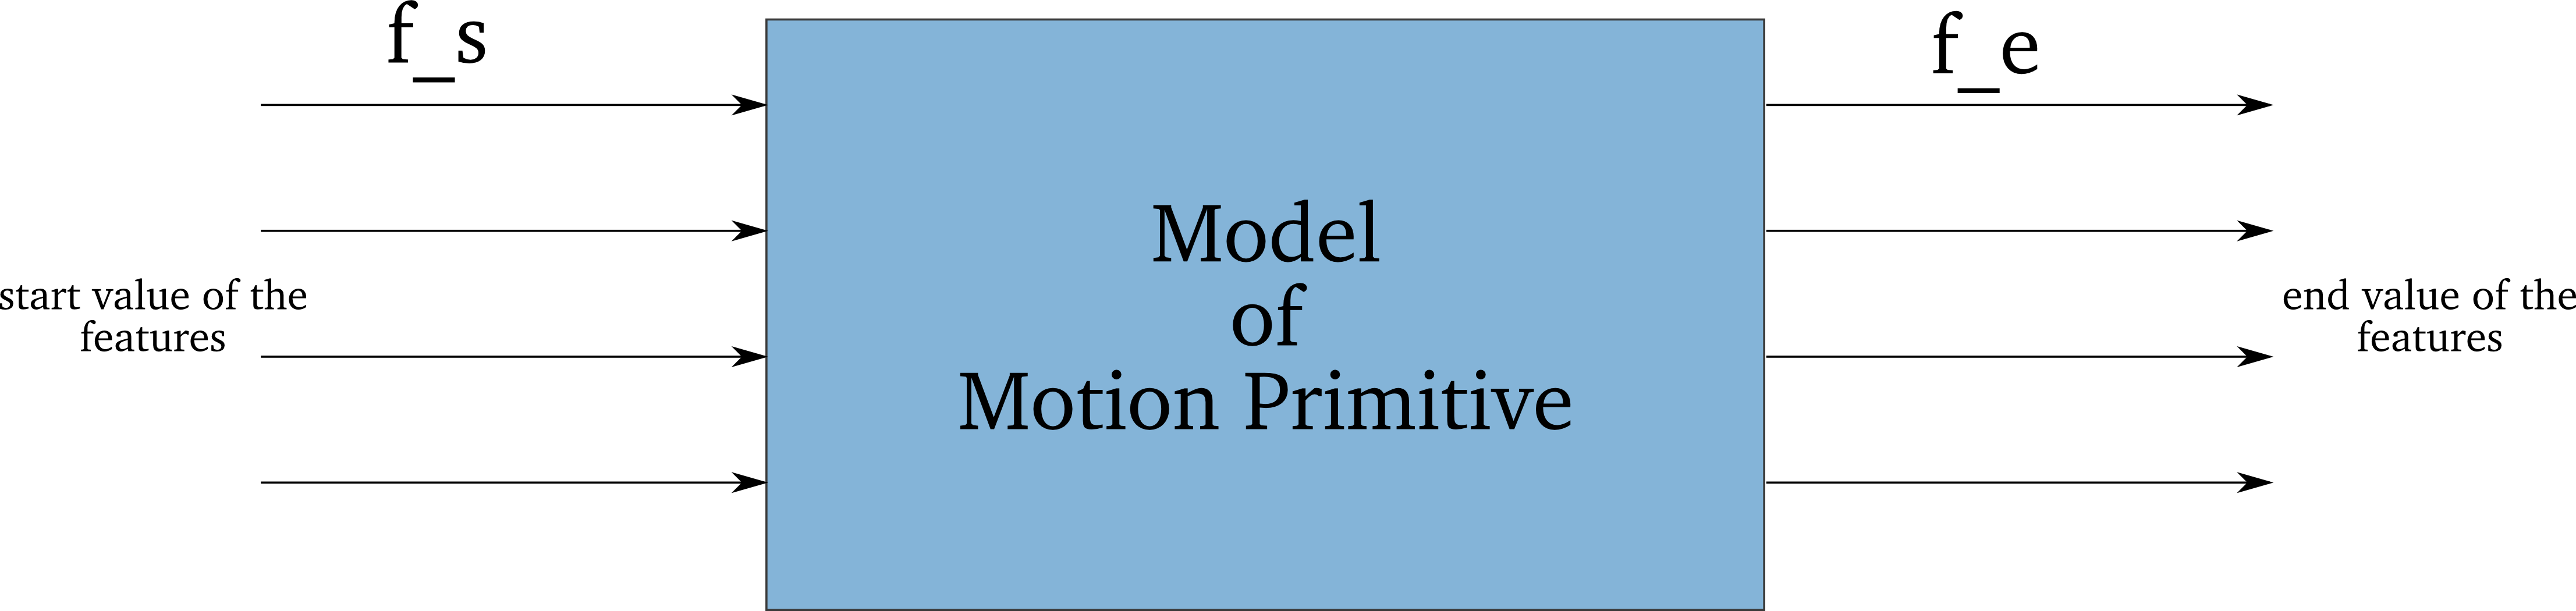
\includegraphics[scale=0.40]{images/model.png}
\caption{Model of motion primitive}
\label{model}
\end{figure}

When the number of training set is limited,learning on
 all the features of the world is not a feasible solutions.
 The approach taken here is to find the relevant features on which the 
learning can be made most effectively.
The prespective adopted in finding the relevant features is that in multiple
demonstrations of the same action, some features will share similar values 
in all the demonstrations. Since we are demonstrating a single action
there has to be consistency in some features of the action.
We need to identify these consistent features and these become the relevant
features. The consistency increases the relevance of the feature to
sucessfully predict from new unseen start states.

We will consider a bivariate probability density function $\phi_i$  by
considering 2 variables, the value of a feature in start of demonstration and
its value at the end of the demonstration.

Let $s_i$ be the $i^{th}$ feature of $f_s$, 
and $e_i$ be the $i^{th}$ feature of $f_e$, \\
The bivariate distribution is given by :
\begin{equation}
    \phi_i(s_i , r_i) = \eta_i I_i ( \lfloor s_i \rfloor, \lfloor e_i \rfloor)
\end{equation}
where operator $\lfloor .  \rfloor$ is  a quantization operator, that returns the bin unit in 
the histogram $I_i$, that corresponds to the feature.

The bi-variate distribution is an appropriate criteria to comment on the
relevance of the feature. Using the distribution we can conclude on the
convergence of the feature. A feature which has converged, the final values
will lie on a straight line in the distribution. If all the final values lie on
a straight line it ensures that whatever maybe the initial value the end values
always remain constant. The constant value in all the demonstration concludes
that the corresponding feature is relevant with respect to the intent of the
motion primitive.
This is explained in the figure \ref{fig:feature distribution}. Higher the
degree of convergence, higher the relevance of the feature for the motion
primitive.
\begin{figure}
    \centering
    \begin{subfigure}[b]{0.4\textwidth}
        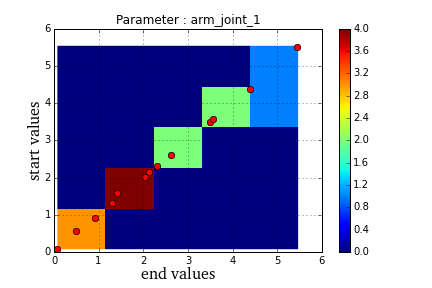
\includegraphics[scale=0.5]{images/arm_joint_1JoinPDF.png} 
        \caption{Distribution of the feature describing arm joint 1.}
        \label{sub fig 1}
    \end{subfigure}
    \begin{subfigure}[b]{0.4\textwidth}
        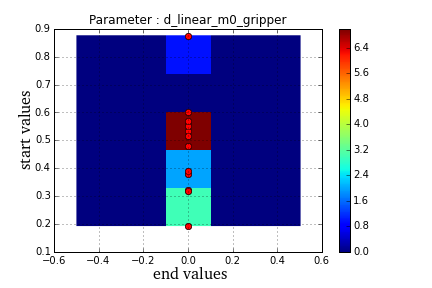
\includegraphics[scale=0.5]{images/d_linear_m0_gripperJoinPDF.png} 
        \caption{Distribution of feature describing distance of object 0 and tooltip. }
        \label{sub fig 2}
    \end{subfigure}
    \caption[Bivariate distribution of features]{An example of bivariate
        distributions of two features for the \textit{move} arm relative to object motion
        primitive.The x-axis is the end values of demonstration while the 
        y-axis is the start value of the demonstration. The dots are the 
        feature values across 12 demonstrations.
        Based on the distribution in \ref{sub fig 1}, we can say that
        there is no certaininty in the end values. This 
        results in lower relvance to the motion primitive . Based on the
        distribution in \ref{sub fig 2},we can say that the end states are
        more concentrated.This ensures that for any value in the start state
        we are sure that the end values always remain same.
        This results in a higher relevance with respect to the motion
    primitive.}\label{fig:feature distribution}
\end{figure}

To calculate this relevance in the distribution, we use two different 
measuring  methods. 1) Entropy 2) Conditional entropy.
We compute the 
entropy $H_i$ and conditional entropy $CH_i$ of the bi-variate distribution $\phi_i(s_i, r_i)$.

Entropy of a discrete random variable is given by,
\begin{equation}
    H(X) = - \sum P(X) \log P(X)
\end{equation}


For a pair of discrete random variables X and Y, which are co related 
conditional entropy of X given Y $h(X|Y)$ is given by :
\begin{equation}
    H(X|Y) =  - \sum _{k = -K}^{K} p_X(x|y) p_Y(y|x) \log \frac{p_Y(y|x)}{p_X(x|y) p_Y(y|x)}
\end{equation}


Based on the entropy or conditional entropy we define the model relevance of a motion primitive.
\begin{equation}
    p(f | \theta ) = \prod_i e^{-E_i}
\end{equation}
where $\theta$ is the set of all $\phi$, and $E_i$ can be $H_i$ or $CH_i$



\subsection{Expert knowledge base}
In our work we create the knowledge base based on expert knowledge of the tasks being performed.
An individual subset of feature space $F$ is called as a template $t$. $t_i \subset F $ .
For example the template $t_1$ contains all the features describing the joint angles of the robot, template $t_2$ contains features which describes 
distance of tooltip to manipulated object.

A collection of the templates is called as a knowledge base $K$.


$K = t_1 \and t_2 \ldots t_n $


\begin{figure}[htp]
\centering
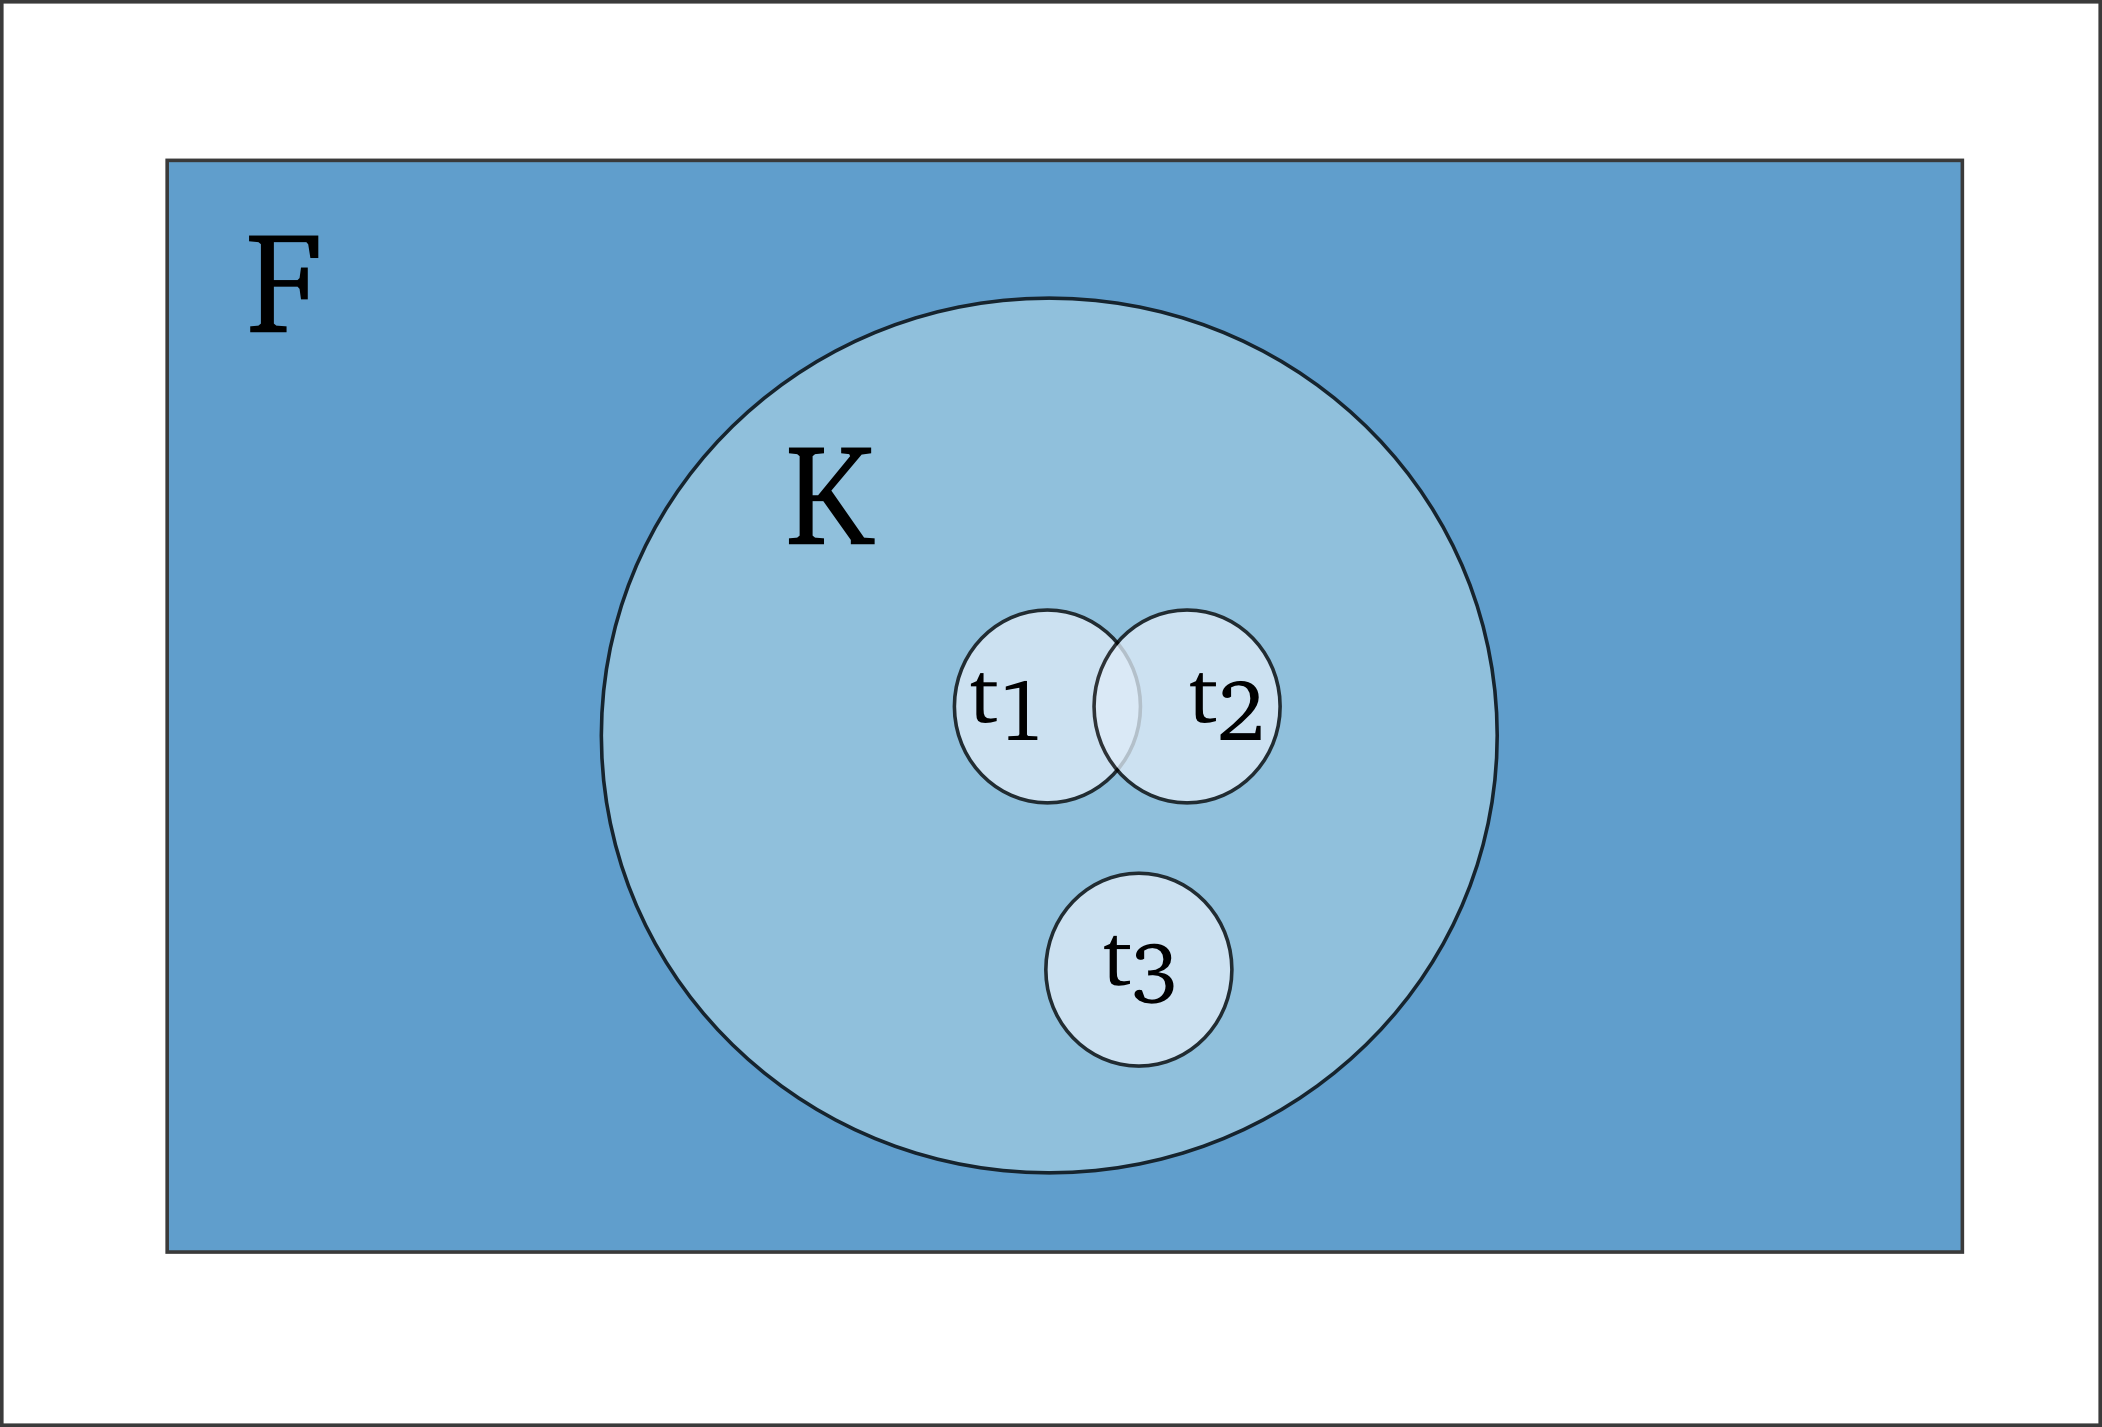
\includegraphics[scale=0.50]{images/feature_space.png}
\caption[Feature space venn diagram]{Relation between feature space F, knowledge base K and the templates t}
\label{}
\end{figure}
Thus for each template $t_i$ we have created a low dimension subset of the feature space $F$.
Our aim is not to find minimum set of features but to find relevant set of features which can describe an action.


The novelty in our approach is the representation of the expert knowledge base.
The knowledge base has been structured using the effect metrics. 
The templates in the knowledge base are organised on the basis of the effect metrics.
The structured nature of the knowledge base helps in determining the relevant features with
less number of demonstrations.
\subsubsection{Effect Metrics}
Effects are defined as changes to the robot-world relationship and/or to positions, orientations
and states of external objects and robot \cite{alissandrakis_action_2006}

In this work we only consider changes to the robot-world relationship and changes to positions, orientations and states of the robot. Based on the orientation and position of the 
robot in environment 2 types of effect metrics can be used, \textit{position} and \textit{orientation}

\begin{figure}[htp]
\centering
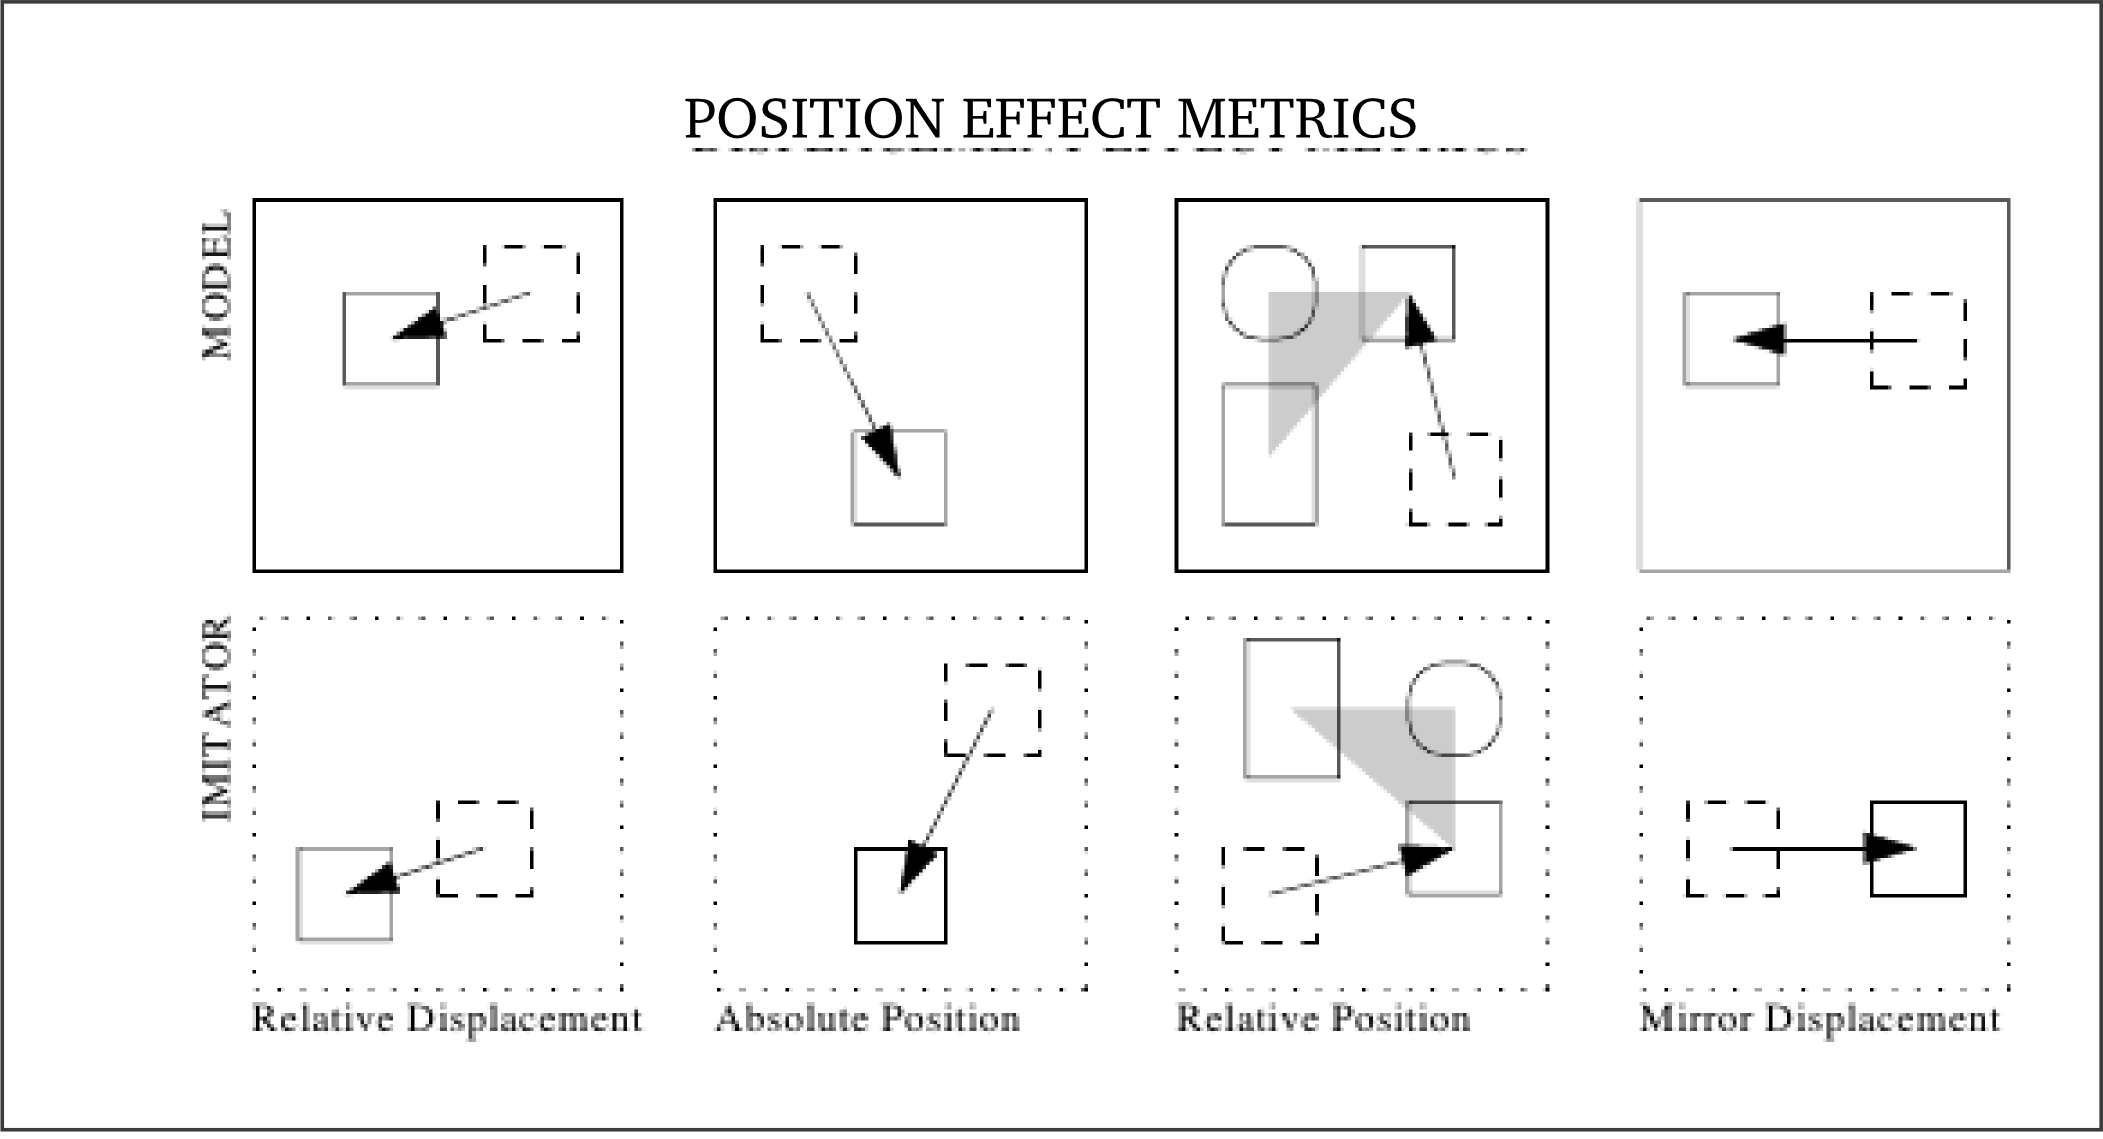
\includegraphics[scale=0.70]{images/position_effect_metrics.png}
\caption[Position effect metrics]{Position effect metrics.
 To measure the change in the relation of change in positions between 
robot and environment objects 
\textit{relative displacement, absolute position, relative position and mirror position}
 effect metrics can be used. First row shows the demonstration and
 their resulting effects. The second rows represents the
 corresponding object (in different workspace ) how it needs to be
 moved (from dashed to solid outline) by an imitator to match the 
corresponding effects according to the metric. The grey triangle
 are superimposed to show the relative position of the objects are 
the same in final state. \cite{alissandrakis_action_2006} }
\label{position effect metrics}
\end{figure}
\begin{figure}[htp]
\centering
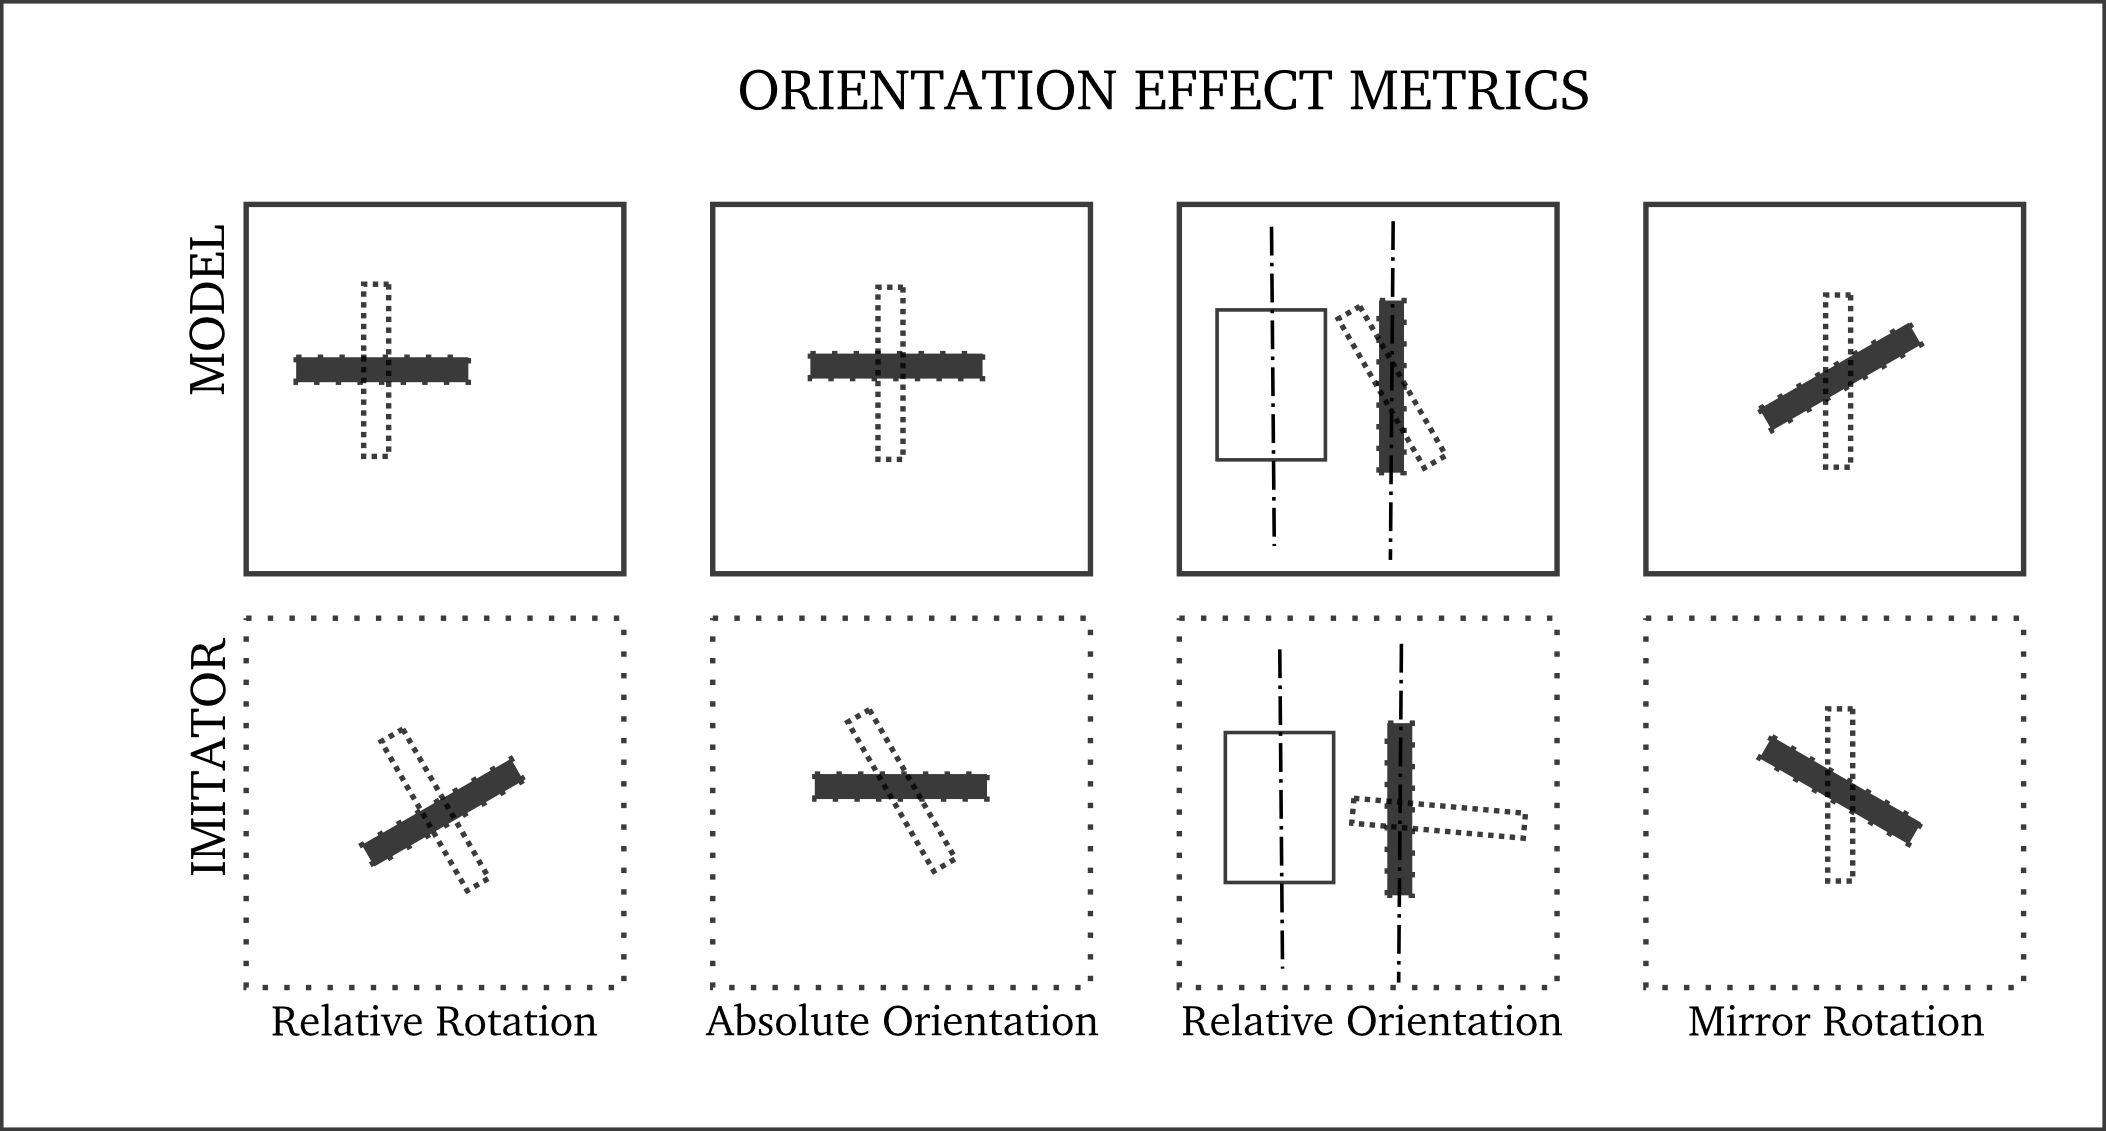
\includegraphics[scale=0.70]{images/angular_effect_metrics.png}
\caption[Orientation effect metrics]{Orientation effect metrics.  To measure the change in the relation of change in orientation between robot and environment objects \textit{relative rotation, absolute orientation, relative orientation and mirror rotation} effect metrics can be used.First row shows the demonstration and their resulting effects. The second rows represents the corresponding object (in different workspace) how it needs to be moved. (from dashed to solid outline) by an imitator to match the corresponding effects according to the metric. The guide lines are superimposed to show the relative orientation of the objects are the same in final state. \cite{ alissandrakis_action_2006}}
\label{orientation effect metrics}
\end{figure}

The different position metrics are 
\begin{itemize}
	\item relative displacement
	\item absolute position
	\item relative position
	\item mirror position
\end{itemize}

the different orientation metrics are 
\begin{itemize}
	\item relative rotation
	\item absolute orientation
	\item relative orientation
	\item mirror rotation
\end{itemize}

Depending on the effect metric the same demonstration can be interpreted as different. 
The example in figure \ref{effect metrics} explains this.
\begin{figure}[htp]
\centering
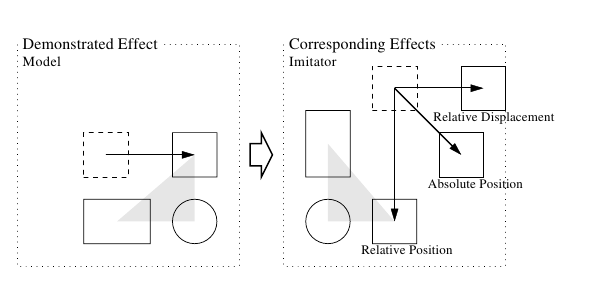
\includegraphics[scale=0.8]{images/effect_position.png}
\caption[Effect metrics in imitation]{The figure illustrates three examples
 of the imitation based on a single demonstration. The left box is the
 demonstrated action. The right box is the possible final state based on
 the position metrics used. The grey triangles are superimposed to show
 the relative distance is maintained \cite{alissandrakis_action_2006}}
\label{effect metrics}
\end{figure}

Based on the effect metrics the knowledge base is organized in different templates which describe an action.
The templates developed in this work are categorized based on the effect metrics.

\subsection{Selecting template from the knowledge base}
For computing the relevance, we use a 3 stage procedure:
\begin{enumerate}
    \item Comparing mean of start value and end value of the feature. $\rightarrow$ To determine that the feature has changed.
            (This was used because features which were not changed in demonstration also have low entropy. So to remove these features this condition 
            check was introduced.)
    \item Comparing the standard deviation of start value and end value of the featue $\rightarrow$ To determing the feature shows convergence in information.
            (This was used because there were features which changed and had low entropy but they were divergent in nature. So to remove the effect of 
            these features this condition check was introduced as explained in figure \ref{fig:box plot})
    \item Calculating the entropy/conditional entropy of the final value of features whose values have changed.
\end{enumerate}

\begin{algorithm}[H]
 \KwData{\\ $f_s$ : start value of the features \\
         $f_e$ : end value of the features\\
        K : knowledge base }
 \KwResult{\\ relevance $L$ of each Template }
 R=0\;
 \For{each template $t$ in K}{
    \For{each feature $f$ in $t$ }{
  read start values $s$ of feature $f$ from $f_s$\;
  read end values $e$ of featue $f$ from $f_e$\;
  \If{mean(s) equals mean(e)}{
       $ R += 1$\;
   }
   \If{standard deviation(s) is less or equal to standard deviation(e)}{
       $ R += 1$\;
   }
    $R += \text{entropy(e)} or\text{ conditional entropy}(e|s)$\;
  }
 }
 \caption{Algorithm for computing relevance of the templates in knowledge base}
\end{algorithm}

\begin{figure}
    \centering
    \begin{subfigure}[b]{0.3\textwidth}
        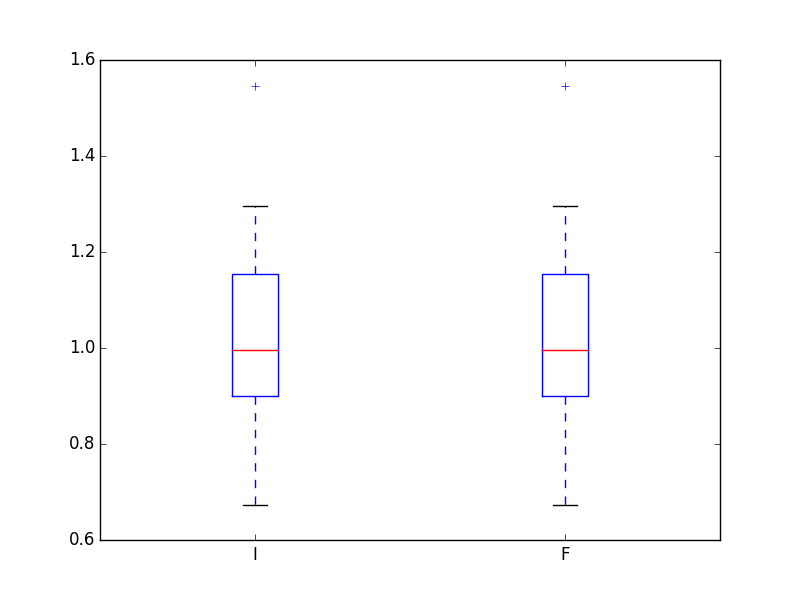
\includegraphics[scale=0.25]{images/boxplot_same_mean.png} 
        \caption{}
        \label{sub box 1}
    \end{subfigure}
    \begin{subfigure}[b]{0.3\textwidth}
        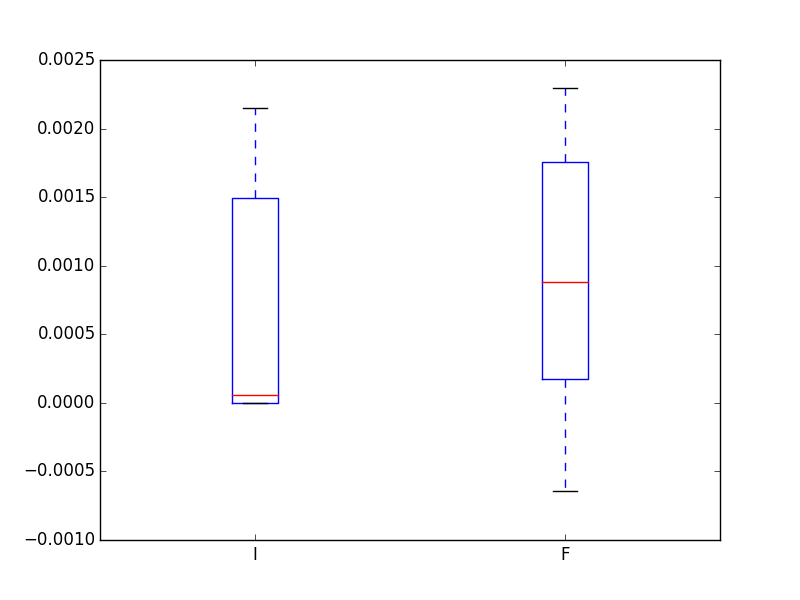
\includegraphics[scale=0.25]{images/boxplot_noconvergence.png} 
        \caption{}
        \label{sub box 2}
    \end{subfigure}
    \begin{subfigure}[b]{0.3\textwidth}
        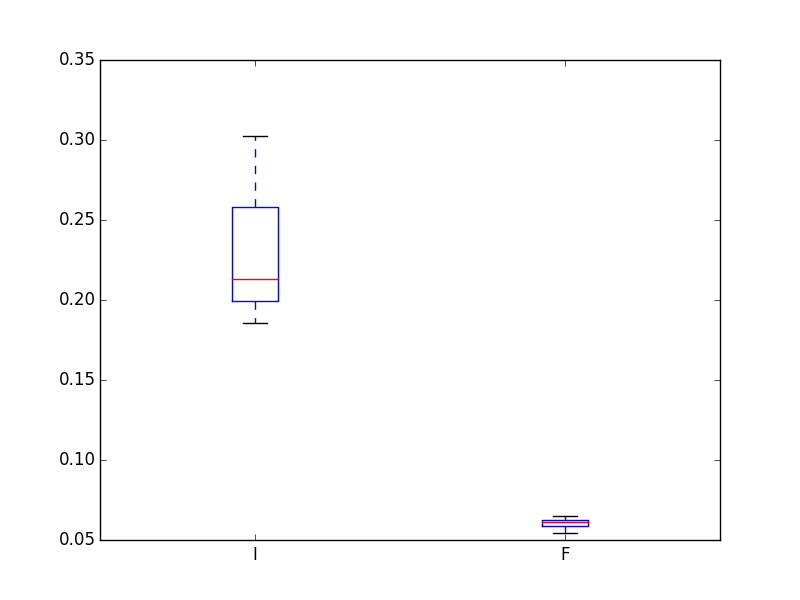
\includegraphics[scale=0.25]{images/boxplot_converged.png} 
        \caption{}
        \label{sub box 3}
    \end{subfigure}
    \caption[Box plot of features]{Box plots of features. Each figure has 2 box plots.
Plot I is of the start value of the feature while plot F is of the end value
of the feature. Figure \ref{sub box 1} is box plot of a featue whose mean values 
have not changed for both start and end values of the feature .
Figure \ref{sub box 2} is the box plot of a feature whose mean value 
has changed but the final values has not converged. 
Figure \ref{sub box 3} is the box plot of a feature whose mean value 
has changed and the final values have converged.} \label{fig:box plot}
\end{figure}


For each $t_i \in K $, we compute a score $\beta_i$ that combines model fitting and the number of 
features in the template.
\begin{equation}
    \beta_i = -2 \log (p (f | \theta_i)) - \alpha_i L_i
\end{equation}
where $\theta_i$ are the distributions related to the features of $t_i$
and $L_i$ is the number of features in the template.
The first term of equation  computes relevance and the second term, weighted by $\alpha$, encourages the usage of templates
consisting of a large number of features $L_i$ .


The most relevant template $T^*$ is selected as :
\begin{equation}
    T^* = \operatornamewithlimits{argmin}_i (\beta_i)
\end{equation}
